%%%%%%%%%%%%%%%%%%%%%%%%%%%%%%%%%%%%%%%%%
% Short Sectioned Assignment
% LaTeX Template
% Version 1.0 (5/5/12)
%
% This template has been downloaded from:
% http://www.LaTeXTemplates.com
%
% Original author:
% Frits Wenneker (http://www.howtotex.com)
%
% License:
% CC BY-NC-SA 3.0 (http://creativecommons.org/licenses/by-nc-sa/3.0/)
%
%%%%%%%%%%%%%%%%%%%%%%%%%%%%%%%%%%%%%%%%%

%----------------------------------------------------------------------------------------
%	PACKAGES AND OTHER DOCUMENT CONFIGURATIONS
%----------------------------------------------------------------------------------------

\documentclass[paper=a4, fontsize=11pt]{scrartcl} % A4 paper and 11pt font size

\usepackage[T1]{fontenc} % Use 8-bit encoding that has 256 glyphs
\usepackage{fourier} % Use the Adobe Utopia font for the document - comment this line to return to the LaTeX default
\usepackage[english]{babel} % English language/hyphenation
\usepackage{amsmath,amsfonts,amsthm} % Math packages

\usepackage{lipsum} % Used for inserting dummy 'Lorem ipsum' text into the template

\usepackage{sectsty} % Allows customizing section commands
\allsectionsfont{\centering \normalfont\scshape} % Make all sections centered, the default font and small caps

\usepackage{fancyhdr} % Custom headers and footers

% my packages
\usepackage{commath}
\usepackage{mathtools}
\usepackage{graphicx}
\usepackage{algorithm}
\usepackage[]{algpseudocode}
\DeclarePairedDelimiter{\ceil}{\lceil}{\rceil}
\usepackage{tikz}
\usepackage{pgfplots}
\pgfplotsset{compat=newest}
\usetikzlibrary{shapes.geometric,arrows,fit,matrix,positioning}
\tikzset
{
    treenode/.style = {white, circle, draw=black, fill=black, align=center, minimum size=1cm},
    nvnode/.style = {circle, draw=black, align=center, minimum size=1cm},
    optnode/.style = {circle, draw=red, red, align=center, minimum size=1cm},
    subtree/.style  = {isosceles triangle, draw=black, align=center, minimum height=0.5cm, minimum width=1cm, shape border rotate=90, anchor=north}
}
\usepackage{hyperref}
\usepackage{enumitem}
\usepackage{subfigure}
\usepackage{multirow}
\newlist{filedescription}{description}{2}
\setlist[filedescription]{font=\normalfont\normalcolor\bfseries\itshape}

\newlist{paramdescription}{description}{1}
\setlist[paramdescription]{font=\normalfont\normalcolor\itshape}

\pagestyle{fancyplain} % Makes all pages in the document conform to the custom headers and footers
\fancyhead{} % No page header - if you want one, create it in the same way as the footers below
\fancyfoot[L]{} % Empty left footer
\fancyfoot[C]{} % Empty center footer
\fancyfoot[R]{\thepage} % Page numbering for right footer
\renewcommand{\headrulewidth}{0pt} % Remove header underlines
\renewcommand{\footrulewidth}{0pt} % Remove footer underlines
\setlength{\headheight}{13.6pt} % Customize the height of the header

\numberwithin{equation}{section} % Number equations within sections (i.e. 1.1, 1.2, 2.1, 2.2 instead of 1, 2, 3, 4)
\numberwithin{figure}{section} % Number figures within sections (i.e. 1.1, 1.2, 2.1, 2.2 instead of 1, 2, 3, 4)
\numberwithin{table}{section} % Number tables within sections (i.e. 1.1, 1.2, 2.1, 2.2 instead of 1, 2, 3, 4)

\setlength\parindent{0pt} % Removes all indentation from paragraphs - comment this line for an assignment with lots of text

% new commands
\newcommand{\filename}[1]{\textbf{\textit{#1}}}
\newcommand{\funcname}[1]{\textbf{#1}}
\newcommand{\inv}{^{\raisebox{.2ex}{$\scriptscriptstyle-1$}}}
\renewcommand{\vec}[1]{\mathbf{#1}}

\makeatletter
\renewcommand*\env@matrix[1][*\c@MaxMatrixCols c]{%
  \hskip -\arraycolsep
  \let\@ifnextchar\new@ifnextchar
  \array{#1}}
\makeatother

\makeatletter
\def\BState{\State\hskip-\ALG@thistlm}
\makeatother

\DeclareMathOperator*{\argmin}{arg\,min} % Jan Hlavacek

%----------------------------------------------------------------------------------------
%	TITLE SECTION
%----------------------------------------------------------------------------------------

\newcommand{\horrule}[1]{\rule{\linewidth}{#1}} % Create horizontal rule command with 1 argument of height

\title{	
\normalfont \normalsize 
\textsc{Mathematical foundations of computer graphics and vision} \\ [25pt] % Your university, school and/or department name(s)
\horrule{0.5pt} \\[0.4cm] % Thin top horizontal rule
\huge Exercise 3. MLS For Curves, Meshes and Images\\ % The assignment title
\horrule{2pt} \\[0.5cm] % Thick bottom horizontal rule
}

\author{Dongho Kang \\ \small 16-948-598} % Your name

\date{\normalsize April 2, 2017} % Today's date or a custom date

\begin{document}

\maketitle % Print the title

%----------------------------------------------------------------------------------------
%	README
%----------------------------------------------------------------------------------------

MATLAB R2016b version was used for coding and testing:

\begin{center}
MathWorks, MATLAB R2016b (9.1.0.441655) \\
64-bit (maci64) 
\end{center}

The \filename{code} directory contains the followings:

\begin{filedescription}
	\item [part1\_2.m] script .m file for exercise part 1.2.
	\item [part1\_3.m] script .m file for exercise part 1.3.
	\item [part1\_4.m] script .m file for exercise part 1.4. (optional problem)
	\item [part1\_5.m] script .m file for exercise part 1.5. (optional problem)
	\item [part2.m] script .m file for exercise part 2.
	\item [functions dir] function .m files 
		\begin{filedescription}
			\item [Fx2D.m] function .m file for calculating $f(\vec{x}) = c_0$ for each 2D $\vec{x}$ points on the grid.
			\item [CalC0.m] function .m file for $f(\vec{x}) = c_0$ for given $\vec{x}$ array (subfunction).
			\item [VisCompSigma.m] function .m file for visualization of curve plot (part 1.2) for given value of sigma.
			\item [FxGradFx3D.m] function .m file for calculating $f(\vec{x}) \nabla f(\vec{x})$ for given 3D $\vec{x}$ point array.
			\item [FxGradFx3D\_ANN.m] function .m file for speeding up calculating $f(\vec{x}) \nabla f(\vec{x})$ for given 3D $\vec{x}$ point array.
			\item [FxGradFx3D\_RIMLS.m] function .m file for calculating $f(\vec{x}) \nabla f(\vec{x})$ for given 3D $\vec{x}$ point array using advanced method.
			\item [AffineTransform.m] function .m file for affine transformation.
			\item [SimilarTransform.m] function .m file for similarity transformation.    
			\item [RigidTransform.m] function .m file for rigid transformation. 
			\item [FvToImg.m] function .m file for creating forward warping image.
			\item [BackwardWarp.m] function .m file for creating backward warping image.
		\end{filedescription}
	\item [data dir] Pre-generated data and images for testing.
		\begin{filedescription}
			\item [p\_array.mat] saved control points (part 2).  
			\item [q\_array.mat] saved deformed points (part 2).
		\end{filedescription}
	\item [files dir] provided funtions and files. Several images and .off files were additionally added for testing.   
\end{filedescription}

For running each .m script, check dependencies (especially for \filename{part1\_4.m} and \filename{part1\_5.m}) and adjust parameters first. Note that \textbf{these scripts only work properly in MATLAB R2016b environment.} More details are stated in the \textit{Running} section of each parts.

%----------------------------------------------------------------------------------------
%	PROBLEM 1
%----------------------------------------------------------------------------------------

\section{exercise part 1: Curve and Surface Reconstruction Using MLS}

In this exercise, moving least squares (MLS) were used for reconstruction of curves (part 1.1 and part 1.2) and smoothing meshes (part 1.3, part 1.4, part 1.5): 

\begin{itemize}
\item derivation of the mathematical formula of the MLS based surfaces (part 1.1).
\item implementing the derived $f(x)$ and plotting the curves for the given three data sets (part 1.2). 
\item derivation of $\nabla f(\vec{x})$ and smoothing provided meshes by $\vec{v'} = \vec{v} - f(\vec{x}) \nabla f(\vec{x})$ (part 1.3). 
\item speeding up mesh smoothing by using Approximate Nearest Neighbor Library (part 1.4). 
\item implementing the sharp feature preserving mesh smoothing proposed on the paper "Feature preserving point set surfaces based on non-linear kernel regression".
\end{itemize}  


\pagebreak

%----------------------------------------------------------------------------------------
%	Curve derivation
%----------------------------------------------------------------------------------------
\subsection{Curve derivation}

In the moving least square problem, given $f(\vec{x}) = \vec{b}(\vec{x})\vec{c}$, the local weight function $\phi_i$, and the local functions $f_i(\vec{x})$, the local error function is defined as follows:

\begin{equation}
\begin{split}
	E_\vec{x}(\vec{c}) &= \sum_{i} \phi_i (\vec{x}) \big( f(\vec{x_i}) - f_i \big) ^2 \\ 
	&= \sum_{i} \phi_i (\vec{x}) \big( \vec{b}(\vec{x_i})^T\vec{c} - f_i \big) ^2	
\end{split}
\end{equation}

In this problem, define $\vec{c}$ and $\vec{b}$ as $\vec{c} = c_0$ and $\vec{b} = 1$ as the exercise instruction suggested. Concerning the local weight function $\phi_i(\vec{x})$ and the local functions $f_i(\vec{x})$, gaussian weight function $\phi_i(\vec{x})$ and reproduced local functions are used:
\begin{align}
	\phi_i(\vec{x}) &= \exp \Big( - \frac{\norm{\vec{x} - \vec{x_i}} ^2}{\sigma^2} \Big) \\
	f_i(\vec{x}) &= \vec{n_i}^T (\vec{x} - \vec{x_i}):
\end{align}
Thus, the moving least square problem can be described as follows:

\begin{equation}
	\argmin_{c_0} E_{\vec{x}}(c_0) = \argmin_{c_0} \sum_i \exp \Big( - \frac{\norm{\vec{x} - \vec{x_i}} ^2}{\sigma^2} \Big) \big(c_0 - \vec{n_i}^T(\vec{x} - \vec{x_i}) \big)^2 
\end{equation}

The closed form solution can be obtained by differentiation:
\begin{gather}
	\frac{\,d E_\vec{x}(c_0)}{\,d c_0} = \sum_{i} 2 \exp \Big( - \frac{\norm{\vec{x} - \vec{x_i}} ^2}{\sigma^2} \Big) \big( c_0 - \vec{n_i}^T(\vec{x} - \vec{x_i}) \big) = 0 
	\\
	\sum_{i} \exp \Big( - \frac{\norm{\vec{x} - \vec{x_i}} ^2}{\sigma^2} \Big) c_0 = \sum_{i} \exp \Big( - \frac{\norm{\vec{x} - \vec{x_i}} ^2}{\sigma^2} \Big) (\vec{n_i}^T(\vec{x} - \vec{x_i}))
\end{gather}

\begin{equation}
	f(\vec{x}) = c_0 = \frac{\sum_{i} \exp \big( - \frac{\norm{\vec{x} - \vec{x_i}} ^2}{\sigma^2} \big) \big( \vec{n_i}^T(\vec{x} - \vec{x_i}) \big) }{\sum_{i} \exp \big( - \frac{\norm{\vec{x} - \vec{x_i}} ^2}{\sigma^2} \big)}
\end{equation}


%----------------------------------------------------------------------------------------
%	Curves plotting
%----------------------------------------------------------------------------------------
\subsection{Curves plotting}

%----------------------------------------------------------------------------------------
\subsubsection{Description}

As $f(\vec{x})$ was derived in part 1.1, for given 2D sample points and its normal vectors, implicit MLS surface (curve for $\mathbb{R}^2$ domain)can be obtained:

\begin{equation}
S = \{ \vec{x} \mid f(\vec{x}) = 0, \nabla f(\vec{x}) \neq 0 \}	
\end{equation}

For different data sets, and different $\sigma$, $f(\vec{x})$ was calculated for each $\vec{x}$ which is generated by the MATLAB function \funcname{meshgrid} and it was visualized as a color map. The implicit MLS surfaces are described as set of the points which of the value of $f(\vec{x})$ is $0$. These points represent fitted curve.  

%----------------------------------------------------------------------------------------
\subsubsection{Running}

Run the script \filename{part1\_2.m} after setting the parameter \textit{sigmas} for $\sigma$ value. 

%----------------------------------------------------------------------------------------
\subsubsection{Result}

The data sets which contains 2D sample point coordinates and normal vectors were tested: 

\begin{figure}[H]
\caption{Visualization of the data sets\label{fig:simple}}
\noindent\makebox[\textwidth]{
  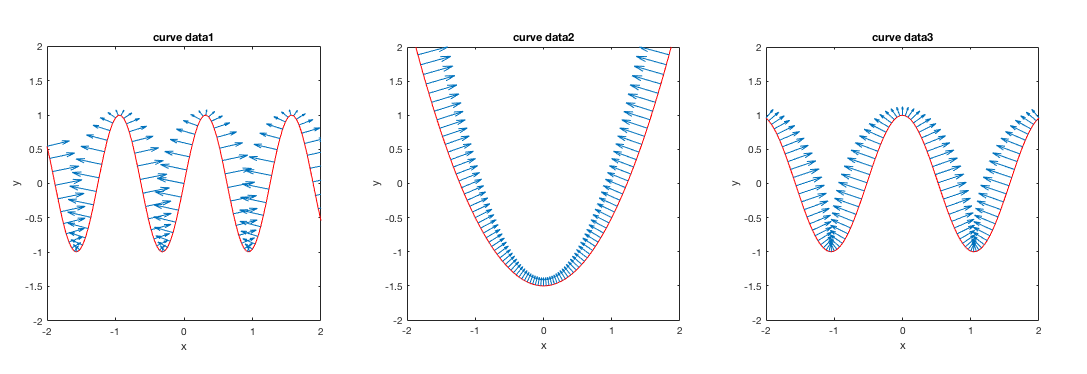
\includegraphics[width=0.85\textwidth]{curve_data_sets}
}
\end{figure} 

For each data sets, color maps and the fitted curves (green curves) were plotted with different values of $\sigma$:

\begin{figure}[H]
\caption{The color map and fitted curve of data set 1\label{fig:simple}}
\noindent\makebox[\textwidth]{
  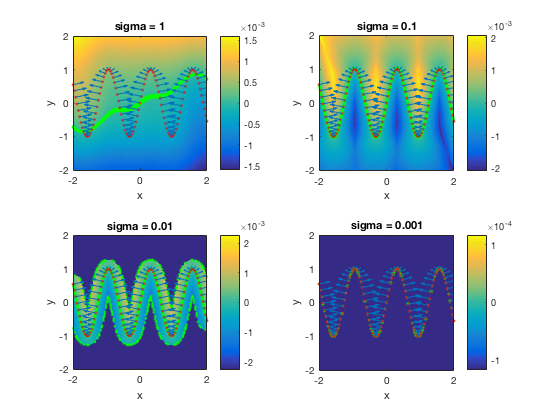
\includegraphics[width=0.85\textwidth]{curve_data1}
}
\end{figure} 
\begin{figure}[H]
\caption{The color map and fitted curve of data set 2\label{fig:simple}}
\noindent\makebox[\textwidth]{
  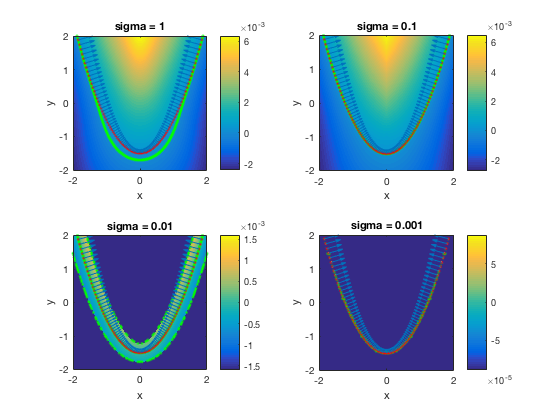
\includegraphics[width=0.85\textwidth]{curve_data2}
}
\vspace*{-0.5in}
\end{figure} 
\begin{figure}[H]
\caption{The color map and fitted curve of data set 3\label{fig:simple}}
\noindent\makebox[\textwidth]{
  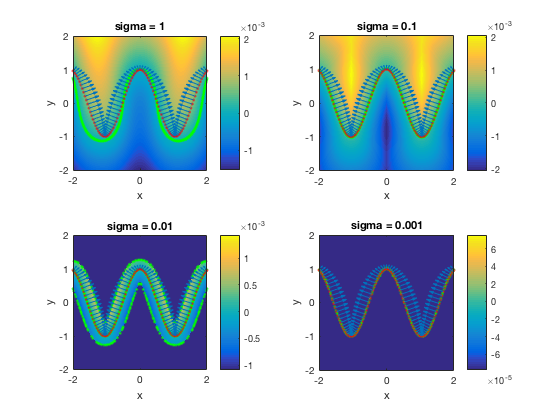
\includegraphics[width=0.85\textwidth]{curve_data3}
}
\end{figure} 
%----------------------------------------------------------------------------------------
\subsubsection{Discussion}

\begin{itemize}
	\item for every data sets, \textbf{$\sigma = 0.1$ showed the best result} i.e. the implicit MLS surfaces (curves) were fitted well with sample points with $\sigma = 0.1$.
	\item \textbf{the parameter $\sigma$ corresponds to the moving window size.} 
	\item when sigma becomes smaller than $\sigma = 0.1$, the size of the window is too small to get a proper curve.  
	\item besides, as sigma becomes larger than $\sigma = 0.1$, the size of the window is too large, so the curve does not fit well with sample points.
\end{itemize}
 
%----------------------------------------------------------------------------------------
%	Smoothing meshes
%----------------------------------------------------------------------------------------
\subsection{Smoothing meshes}

%----------------------------------------------------------------------------------------
\subsubsection{Description}


In the part 1.3, mesh smoothing algorithm based MLS algorithm was implemented. The provided mesh data is composed with vertex coordinates(3D sample points) and normals vectors. The projection of each vertex coordinate $\vec{v}$ to the smoothed coordinates of the mesh vertices $\vec{v'}$ follows $\vec{v'} = \vec{v} - f(\vec{x}) \nabla f(\vec{x})$.

\paragraph{Formulation of projection}

The derivation of $f(\vec{x})$ has been done in the part 1.1 (the equation 1.7). As taking gradient to $f(\vec{x})$, $\nabla f(\vec{x})$ can be obtained as follows:

\begin{equation}
	\begin{split}
		\nabla f(\vec{x}) &= \nabla \frac{\sum_{i} \phi_i(\vec{x}) \big( \vec{n_i}^T(\vec{x} - \vec{x_i}) \big) }{\sum_{i} \phi_i(\vec{x})} 
		\\
		&= \frac{
		\nabla \Big( \sum_{i} \phi_i(\vec{x}) \big( \vec{n_i}^T(\vec{x} - \vec{x_i}) \big) \Big) 
			\big( \sum_{i} \phi_i(\vec{x}) \big) - 
		\Big( \sum_{i} \phi_i(\vec{x}) \big( \vec{n_i}^T(\vec{x} - \vec{x_i}) \big) \Big) \nabla (\sum_{i} \phi_i(\vec{x}))
		}
		{(\sum_{i} \phi_i(\vec{x}))^2}
		\\
		&= \frac{
		\Big( \sum_{i} \phi_i(\vec{x}) \vec{n_i} + \sum_{i} \vec{n_i}^T (\vec{x} - \vec{x_i}) \nabla \phi_i(\vec{x}) \Big) - 
		\big( f(\vec{x}) \sum_{i} \nabla \phi_i (\vec{x}) \big)
		}
		{\sum_{i} \phi_i(\vec{x})}
		\\
		&= \frac{
		\sum_{i} \Big( \phi_i(\vec{x}) \vec{n_i} + \big( \vec{n_i}^T (\vec{x} - \vec{x_i}) - f(\vec{x}) \big) \nabla \phi_i(\vec{x}) \Big)
		}
		{\sum_{i} \phi_i(\vec{x})}
	\end{split}
\end{equation}
	

\paragraph{MATLAB implementation}

Since the formulation for $f(\vec{x}) \nabla f(\vec{x})$ is derived, smoothed coordinates of the mesh vertices $\vec{v'}$ can be calculated with certain value of $\sigma$: $\vec{v'} = \vec{v} - f(\vec{x}) \nabla f(\vec{x})$. After several iterations, $\vec{v'}$ converges. 

\pagebreak

%----------------------------------------------------------------------------------------
\subsubsection{Running}

Run the script \filename{part1\_3.m} after setting the parameters. 

\begin{paramdescription}
\item [sigma\_array] : sigma values for each data sets. Each rows correspond to each data sets.
\item [max\_iter] : the number of maximum iteration. 
\item [threshold] : threshold for convergence. The default value is $10^{-4}$.
\end{paramdescription}


%----------------------------------------------------------------------------------------
\subsubsection{Result}

The result of mesh smoothing with different value of $\sigma$ is as follows:

\begin{figure}[H]
\caption{The smoothed mesh of the bun.off data set\label{fig:simple}}
\centering
\subfigure[original]{
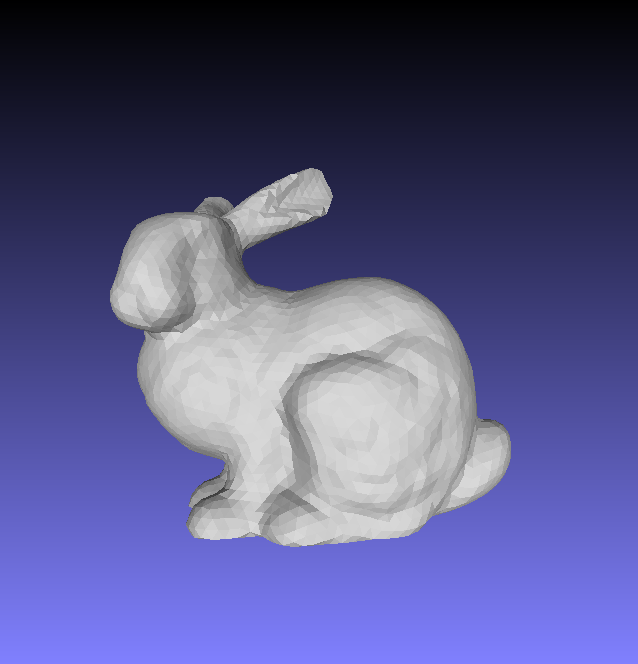
\includegraphics[width=.22\textwidth]{bun}
}
\subfigure[$\sigma = 0.01$]{
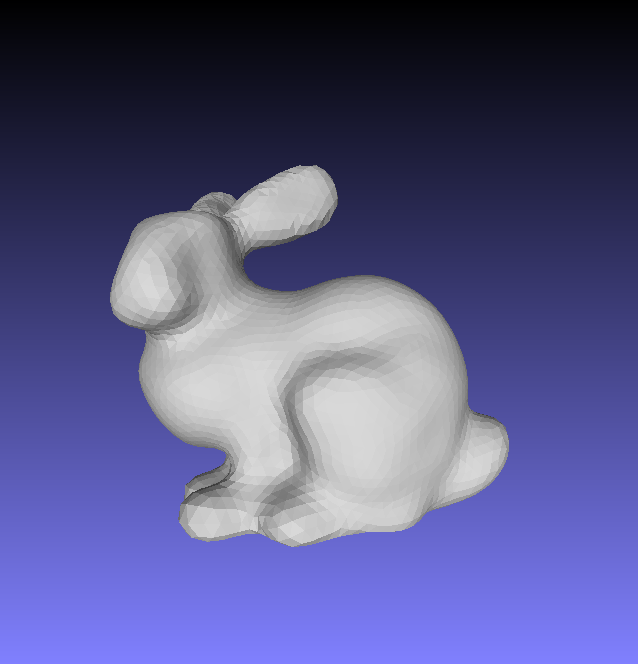
\includegraphics[width=.22\textwidth]{bun_sig001}
}
\subfigure[$\sigma = 0.02$]{
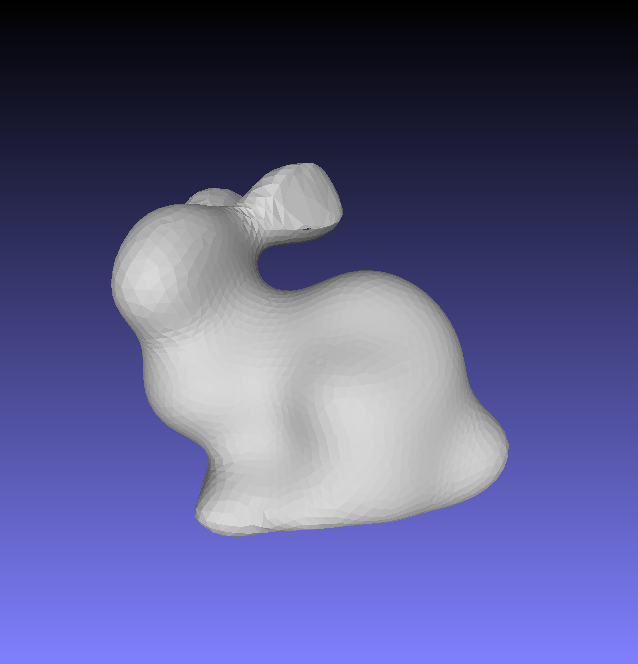
\includegraphics[width=.22\textwidth]{bun_sig002}
}
\subfigure[$\sigma = 0.03$]{
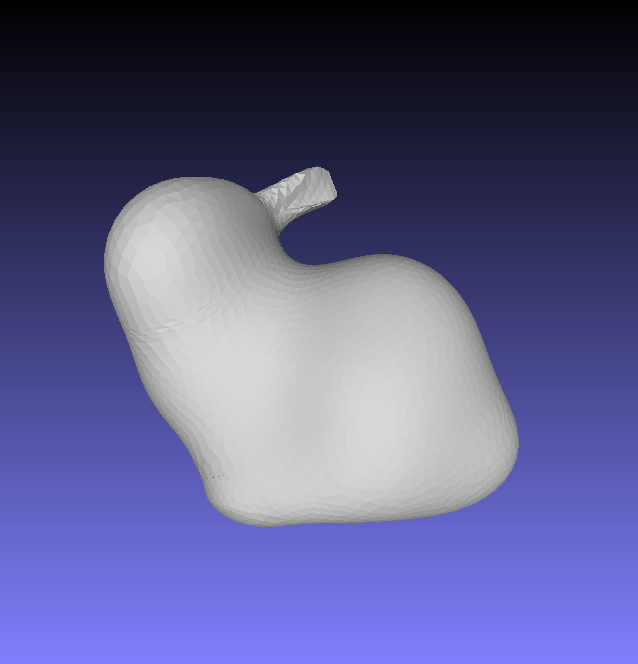
\includegraphics[width=.22\textwidth]{bun_sig003}
}
\end{figure}


\begin{figure}[H]
\caption{The smoothed mesh of the bun.off data set\label{fig:simple}}
\centering
\subfigure[original]{
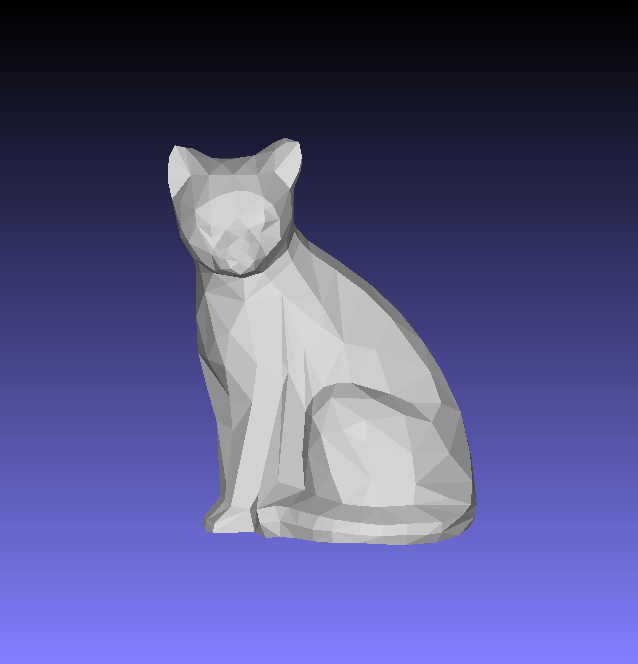
\includegraphics[width=.22\textwidth]{cat}
}
\subfigure[$\sigma = 80$]{
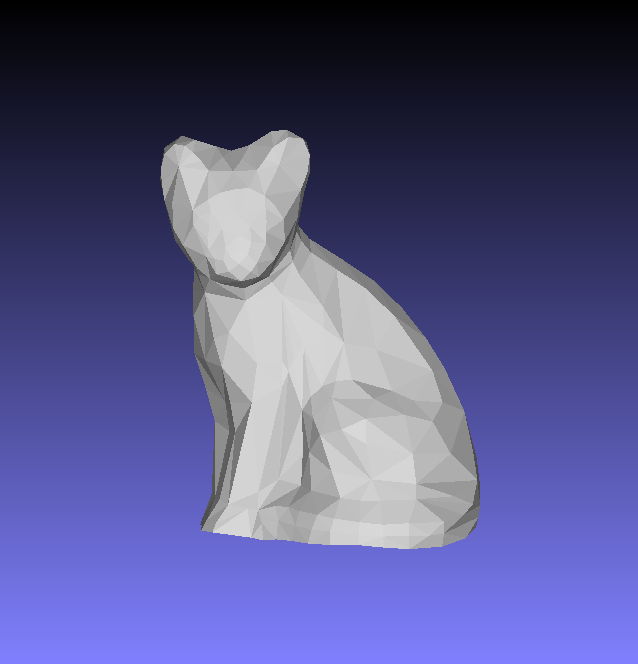
\includegraphics[width=.22\textwidth]{cat_sig80}
}
\subfigure[$\sigma = 90$]{
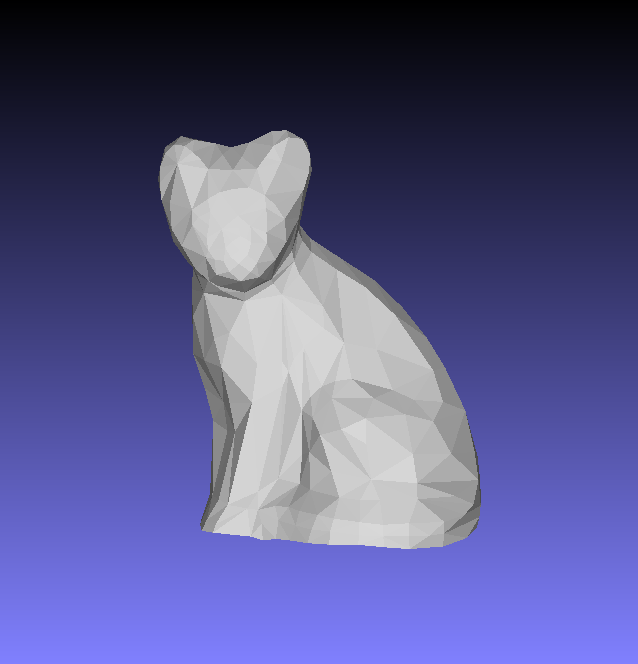
\includegraphics[width=.22\textwidth]{cat_sig90}
}
\subfigure[$\sigma = 100$]{
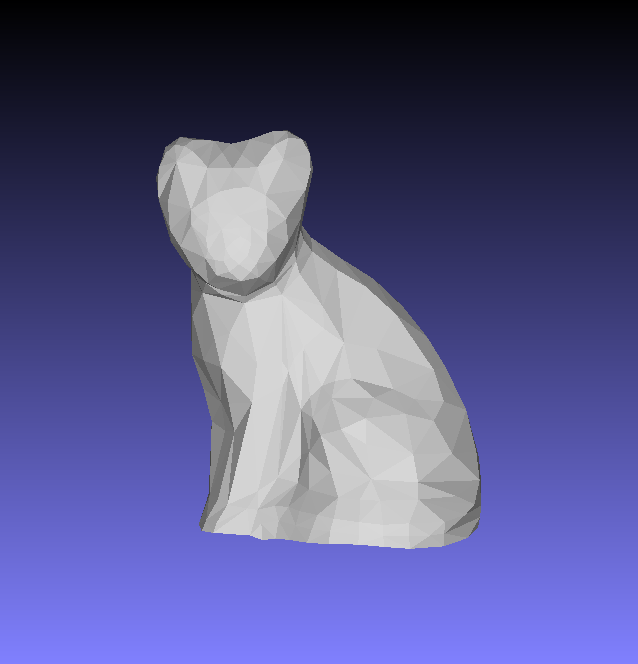
\includegraphics[width=.22\textwidth]{cat_sig100}
}
\end{figure}

%----------------------------------------------------------------------------------------
\subsubsection{Discussion}

\begin{itemize}
	\item comparing the results, \textbf{as $\sigma$ increases, the amount of mesh smoothing increases.} 
	\item remark that the parameter $\sigma$ corresponds to the moving window size. Large value of $\sigma$ means smoothing area is large.
\end{itemize}


\pagebreak

%----------------------------------------------------------------------------------------
%	Speeding up mesh smoothing
%----------------------------------------------------------------------------------------
\subsection{Speeding up mesh smoothing}

%----------------------------------------------------------------------------------------
\subsubsection{Description}

In part 1.4, Approximate Nearest Neighbor Library was used to speed up mesh smoothing. By using the library function \funcname{frsearch}, $f(\vec{x}) \nabla f(\vec{x})$ can be calculated for sample points $3\sigma$ away from the query point $\vec{x}$ only. 

%----------------------------------------------------------------------------------------
\subsubsection{Running}

The MATLAB script \filename{part1\_ 4.m} corresponds to mesh smoothing with ANN library. 

Before running the script, MATLAB ANN wrapper should be installed. Please note the followings. 

\begin{itemize}
\item refer to ANN wrapper github repository: \url{https://github.com/jefferislab/MatlabSupport/tree/master/ann_wrapper}
\item \funcname{randint} function used in ANN wrapper is deprecated in MATLAB 2016b version. If \funcname{randint} function of ANN wrapper library makes error during running time, change it to \funcname{randi}.
\item although changing \funcname{randint} to \funcname{randi}, \filename{test\_ ann\_ class.m} file which included in ANN wrapper library still does not work properly. However \funcname{frsearch} works without any problem. 
\item before running \filename{part1\_4.m} script, add ANN wrapper path.
\end{itemize}

%----------------------------------------------------------------------------------------
\subsubsection{Result}

The running time for each data set with different $\sigma$ is as follows:

\begin{table}[h]
\captionof{table}{The running time of mesh smoothing} \label{tab:title} 
\centering
\begin{tabular}{| c | c | c | c | }
\hline
					File 	& $\sigma$ 	& Normal	& ANN \\
\hline 
\multirow{3}{*}{bun.off}	& 0.01 		& 43.38		& 16.34 	 \\ \cline{2-4}
							& 0.02 		& 36.18		& 47.18 	 \\ \cline{2-4}
							& 0.03		& 40.46		& 115.17	 \\ \hline
\multirow{3}{*}{bunny.off}	& 0.01 		& 34.62		& 12.45  	\\ \cline{2-4}
							& 0.02 		& 34.67		& 46.14  	\\ \cline{2-4}
							& 0.03		& 35.11		& 108.84	 \\ \hline							
\multirow{3}{*}{bunny2.off}	& 0.01 		& 34.90		& 15.28  	\\ \cline{2-4}
							& 0.02 		& 35.72		& 46.41  	\\ \cline{2-4}
							& 0.03		& 36.21		& 129.90	 \\ \hline
\multirow{3}{*}{cat.off}	& 80 		& 1.34 		& 1.66  	\\ \cline{2-4}
							& 90 		& 1.15 		& 1.19  	\\ \cline{2-4}
							& 100		& 1.14 		& 1.23	 	\\ \hline
\end{tabular}
\end{table}

The discussion regarding the result follows on next page.

%----------------------------------------------------------------------------------------
\subsubsection{Discussion}

When $\sigma$ is small, running time is reduced by \funcname{frsearch}, because the number of the points to calculate $f(\vec{x}) \nabla f(\vec{x})$ becomes smaller. However, as $\sigma$ is getting larger, advantage of using \funcname{frsearch} is not considerable anymore. Besides, finding neighboring points becomes overhead in this case, thus, running time even increased than before. 


%----------------------------------------------------------------------------------------
%	Advanced method
%----------------------------------------------------------------------------------------
\subsection{Advanced method}

%----------------------------------------------------------------------------------------
\subsubsection{Description}

In part 1.5, sharp feature preserving mesh smoothing by Robust Implicit Moving Least Squares(RIMLS) method was implemented. In order to reduce the running time, the algorithm was vectorized. \\

Several implementation choices are determined as follows:

\begin{itemize}
	\item 
	for the spatial weight function $\phi_i(\vec{x})$, gaussian function was used. 
	\begin{equation*}
	\phi_i(\vec{x}) = \exp \Big( - \frac{\norm{\vec{x} - \vec{x_i}} ^2}{h_i^2} \Big)
	\end{equation*} 
	\item $h_i$ determined as follows (same value was used for $i = 1, 2, \dots, N$):
	\begin{equation*} h_i = \frac{\sum_{i}^{N} 1.4 \times d_i}{N} \end{equation*}
	where $d_i$ is the minimum distance from sample point $\vec{v_i}$ to other sample points.
	\item $\sigma_r = 0.5$ was used. 
\end{itemize}


%----------------------------------------------------------------------------------------
\subsubsection{Running} 

Before running the script \filename{part1\_5.m}, MATLAB ANN wrapper should be installed. Please refer to part 1.4. \\
Since the results are very sensitive to parameters, they were tuned carefully. Do not change any parameter in the script.

%----------------------------------------------------------------------------------------
\subsubsection{Result}

The following figures are smoothed mesh of the same data set. One is by normal moving least square (Implicit Moving Least Squares; IMLS) which was implemented in part 1.3 and the other is by advanced method, the RIMLS implemented in part 1.5.

\begin{figure}[H]
\caption{Comparison of the smoothed mesh of the bun.off data set\label{fig:simple}}
\centering
\subfigure[original]{
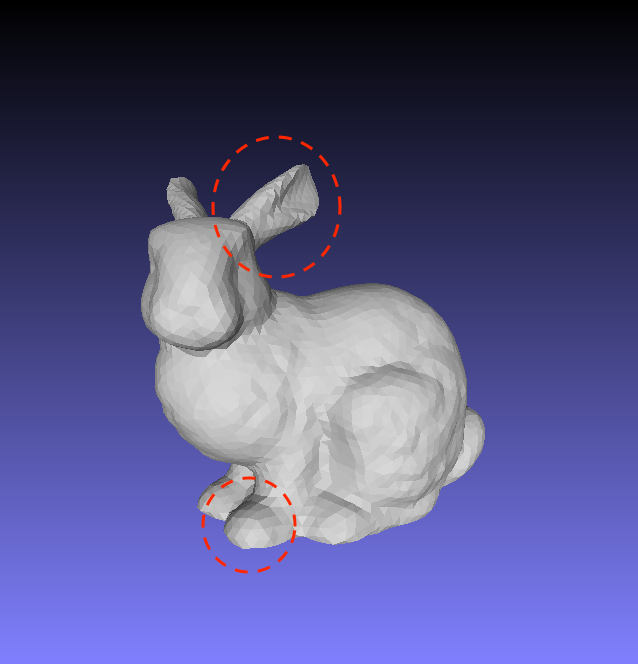
\includegraphics[width=.3\textwidth]{bun_origin}
}
\subfigure[smoothed by normal IMLS]{
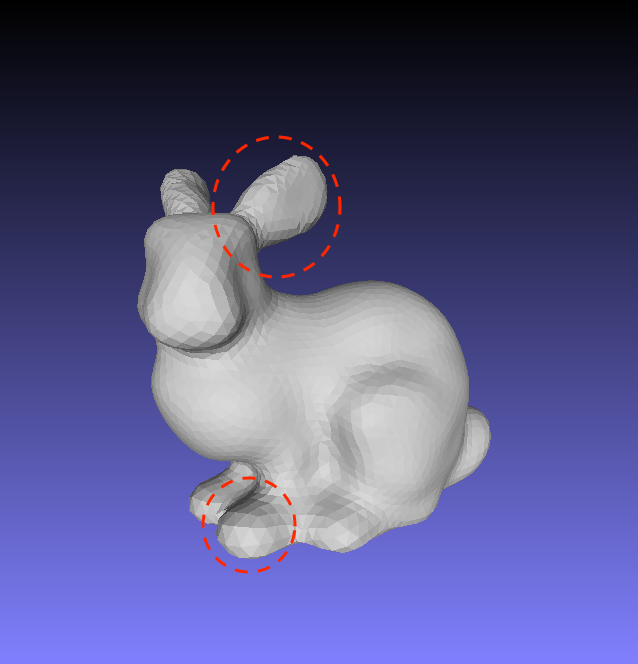
\includegraphics[width=.3\textwidth]{bun_IMLS}
}
\subfigure[smoothed by RIMLS]{
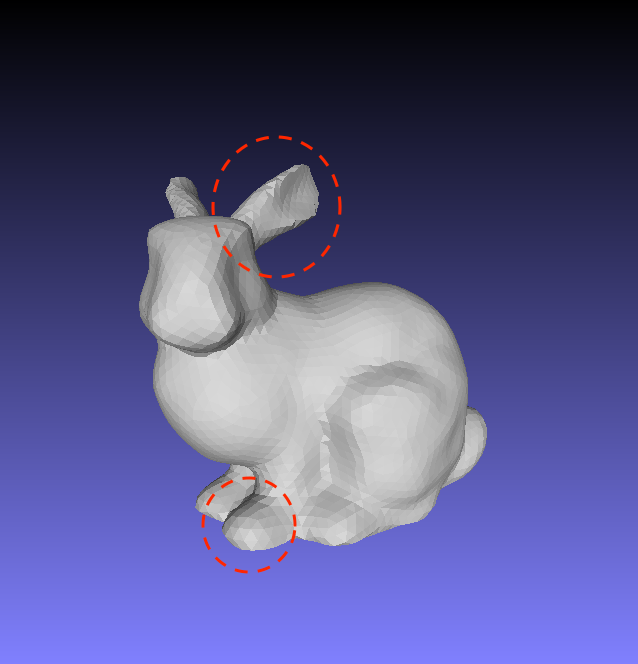
\includegraphics[width=.3\textwidth]{bun_RIMLS}
}
\end{figure}

The differences are salient especially for ear and foot part of the bunny model. The RIMLS smoothes similar amount but preserve sharp edges. 


%----------------------------------------------------------------------------------------
%	PROBLEM 2
%----------------------------------------------------------------------------------------

\section{exercise part 2: Image Deformation Using Moving Least Squares}


%----------------------------------------------------------------------------------------
\subsubsection{Description}

For part 2, moving least square used for image deformation. Three deformation model was adapted:

\begin{itemize}
	\item affine transformation
	\item similarity transformation 
	\item rigid transformation
\end{itemize}

The weights $w_i$ for a control point $\vec{p_i}$, its deformed position $\vec{q_i}$ and an image point $\vec{v}$ is given as:

\begin{equation}
	w_i = \frac{1}{\abs{\vec{p_i} - \vec{v}} ^ {2 \alpha}}
\end{equation}

$p_*$ and $q_*$ are defined as follows:

\begin{align}
	\vec{p_*} &= \frac{\sum_i w_i \vec{p_i}}{\sum_i w_i} \\
	\vec{q_*} &= \frac{\sum_i w_i \vec{q_i}}{\sum_i w_i}  
\end{align}

\paragraph{Affine transformation} 

For affine transformation, deformation function $f_a$ is as follows:

\begin{equation}
	f_a(\vec{v}) = (\vec{v} - \vec{p_*}) \Bigg( \sum_i \vec{\hat{p_i}}^T w_i \vec{\hat{p_i}} \Bigg) \inv w_j \vec{\hat{p_j}}^T
\end{equation} 

\paragraph{Similarity transformation}

For similarity transformation, deformation function $f_s$ is as follows:

\begin{gather}
	f_s(\vec{v}) = \sum_i \hat{\vec{q_i}} (\frac{1}{\mu_s} A_i) + \vec{q_*} \\
	A_i = w_i \Bigg( 
	\begin{array}{c}
		\vec{\hat{p_i}} \\
		- \vec{\hat{p_i}}^\perp
	\end{array} \Bigg) \Bigg(
	\begin{array}{c}
		\vec{v} - \vec{p_*} \\
		- (\vec{v} - \vec{p_*})^\perp
	\end{array} \Bigg)^T
\end{gather}


\paragraph{Rigid transformation}

For similarity transformation, deformation function $f_r$ is as follows:

\begin{equation}
	f_r(\vec{v}) = \sum_i \hat{\vec{q_i}} A_i
\end{equation}

where, $A_i$ is from equation (2.6).

\paragraph{Backward warping}

As deforming image and mapping each 2D point $\vec{v}$ of original image to deformed position $f(\vec{v})$ ($f$ is $f_a$ for affine, $f_s$ for similarity and $f_r$ for rigid transformation), artifacts can be made since deformed image points might be non-integer. In order to avoid these artifacts, backward warping was implemented. \\

Since the value of the deformation function $\vec{v'} = f(\vec{v})$ is obtained for every original image points, the inversed function $f\inv$ can be obtained by regression. With $f\inv$, for each point of deformed image $\vec{v'}$, now $\vec{v} = f\inv(\vec{v'})$ can be calculated. If calculated $\vec{v}$ vector contains non-integer value, simply interpolated to nearest neighbor. For the regression, MATLAB function \funcname{griddata} was used.

\pagebreak

%----------------------------------------------------------------------------------------
%	RUNNING
%----------------------------------------------------------------------------------------
\subsection{Running}

Run the script \filename{part2.m} after setting the parameters. 

\begin{paramdescription}
\item [alpha] : the $\alpha$ value of the weight $w_i$
\item [img\_idx] : 1 for ginger.png as an input, 2 for kerr.jpg
\item [saved\_control\_pts] : for ginger.png, saved control points can be used. (for debugging)  
\end{paramdescription}

%----------------------------------------------------------------------------------------
%	RESULT
%----------------------------------------------------------------------------------------
\subsection{Result}

The results of the deformation with $\alpha = 1$ is as follows. 

\begin{figure}[H]
\caption{ginger.png for different transformation model\label{fig:simple}}
\centering
\subfigure[forward warping]{
	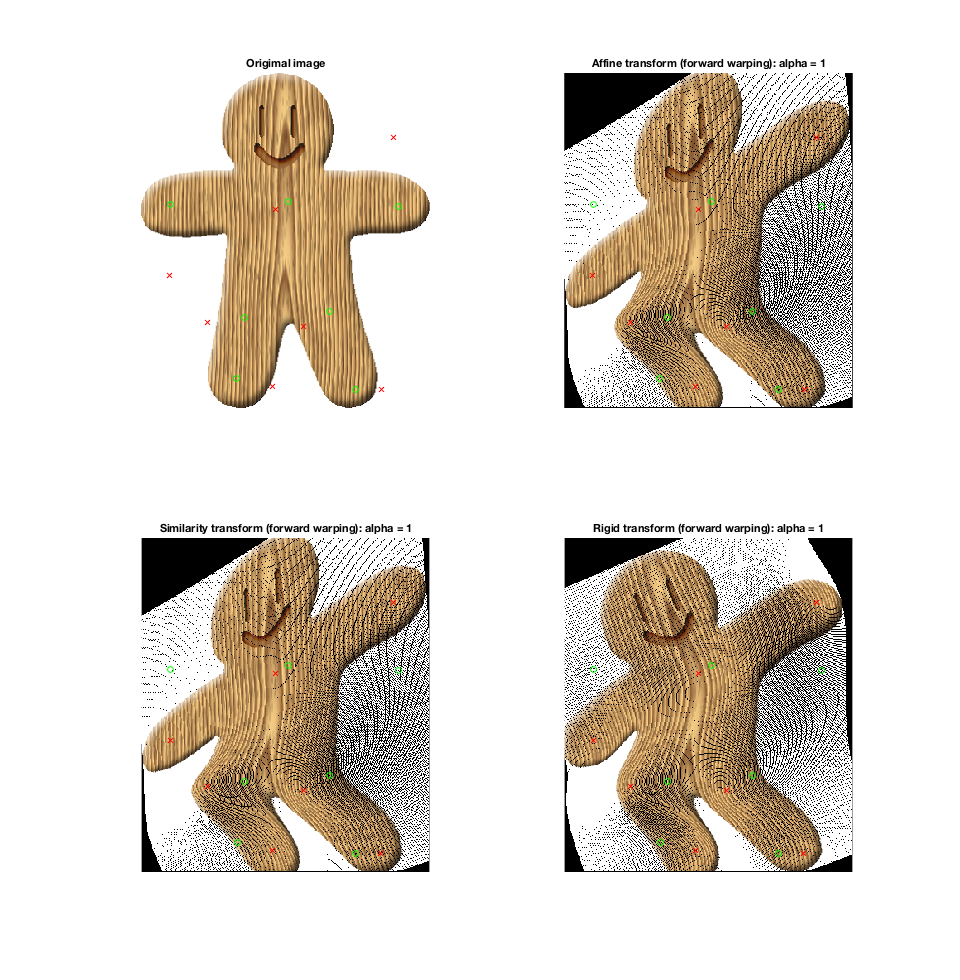
\includegraphics[width=0.4\textwidth]{deformation_forward}}
\subfigure[backward warping]{
  	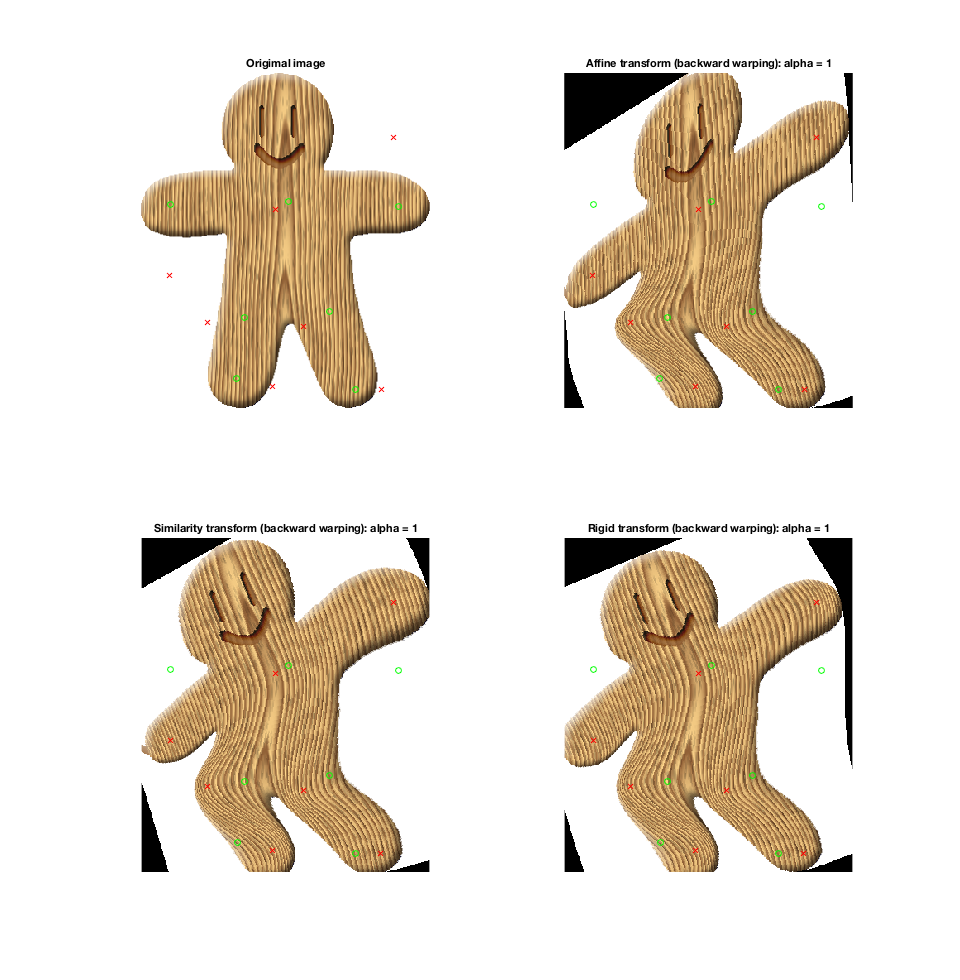
\includegraphics[width=0.4\textwidth]{deformation_backward}}
\end{figure}

Comparing for different value of $\alpha$:

\begin{figure}[H]
\caption{ginger.png with different $\alpha$\label{fig:simple}}
\centering
\subfigure[$\alpha$ = 0.5]{
	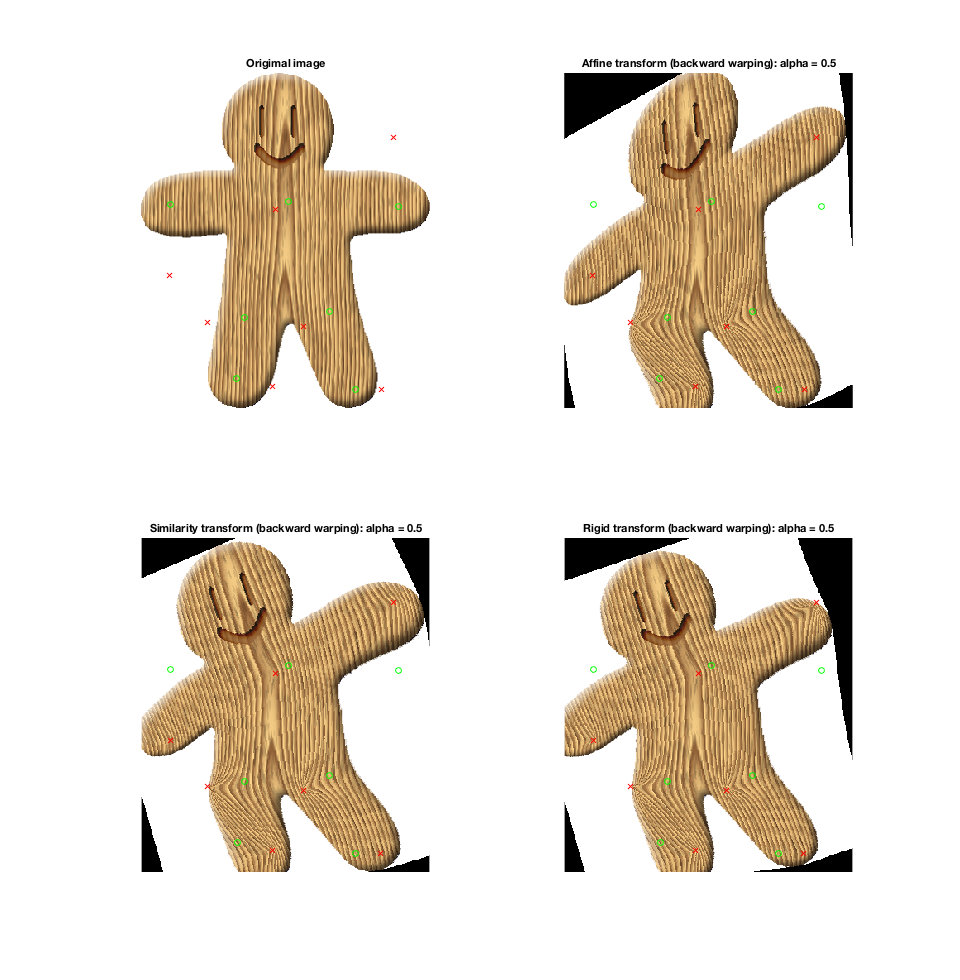
\includegraphics[width=0.3\textwidth]{deformation_backward_alpha05}}
\subfigure[$\alpha$ = 1.0]{
	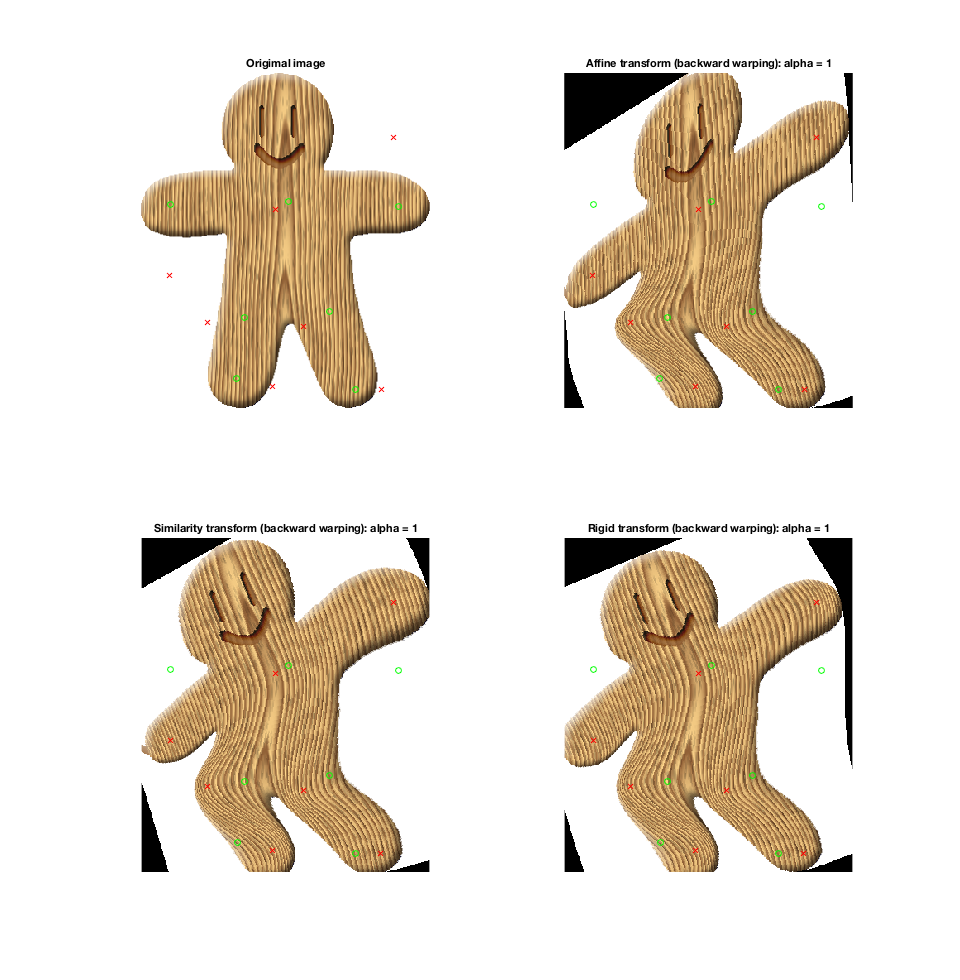
\includegraphics[width=0.3\textwidth]{deformation_backward}}
\subfigure[$\alpha$ = 2.0]{
	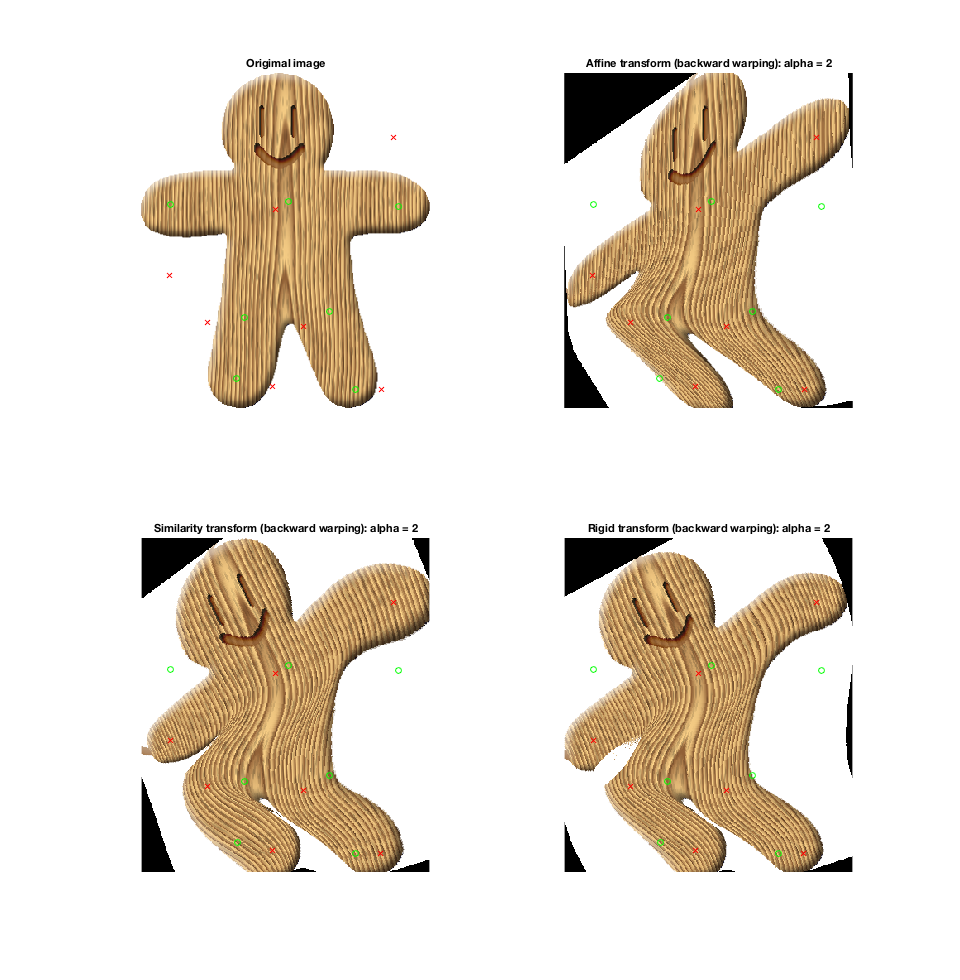
\includegraphics[width=0.3\textwidth]{deformation_backward_alpha2}}
\end{figure}

\begin{figure}[H]
\caption{ginger.png with $\alpha = 0.5, 2.0$ large images\label{fig:simple}}
\centering
\subfigure[$\alpha$ = 0.5]{
	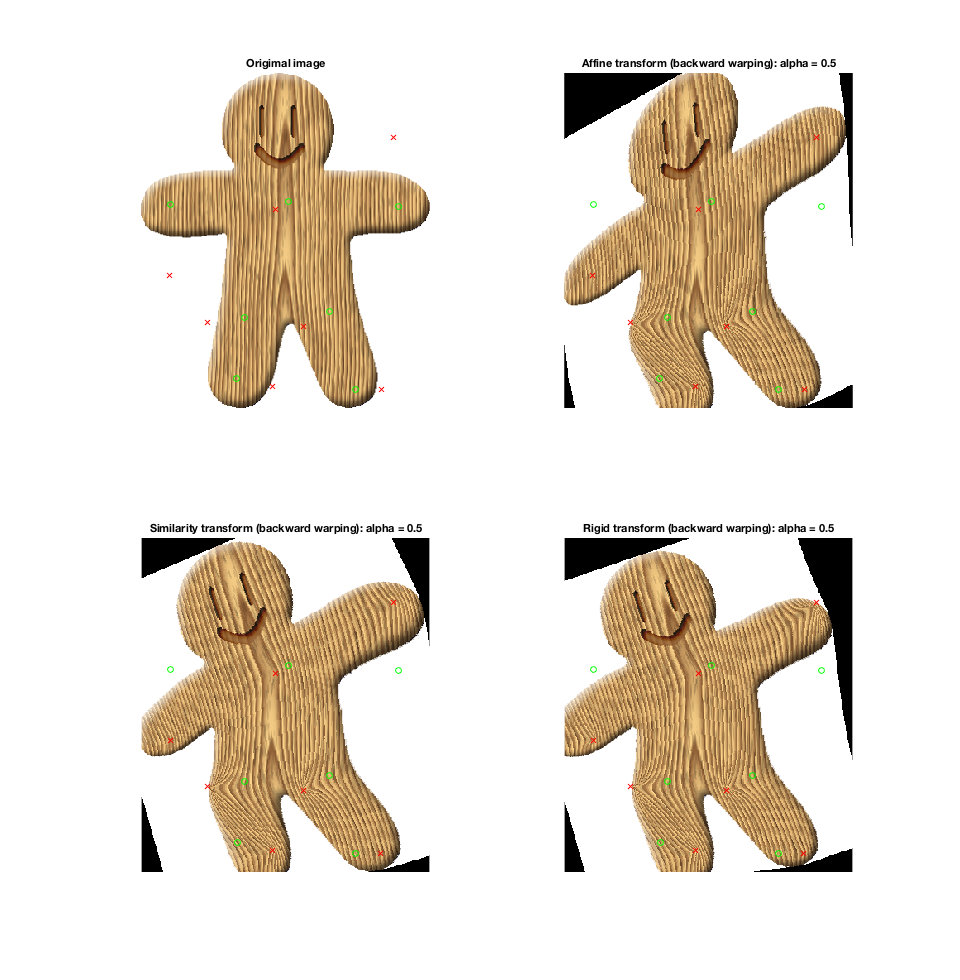
\includegraphics[width=0.7\textwidth]{deformation_backward_alpha05}}
\subfigure[$\alpha$ = 2.0]{
	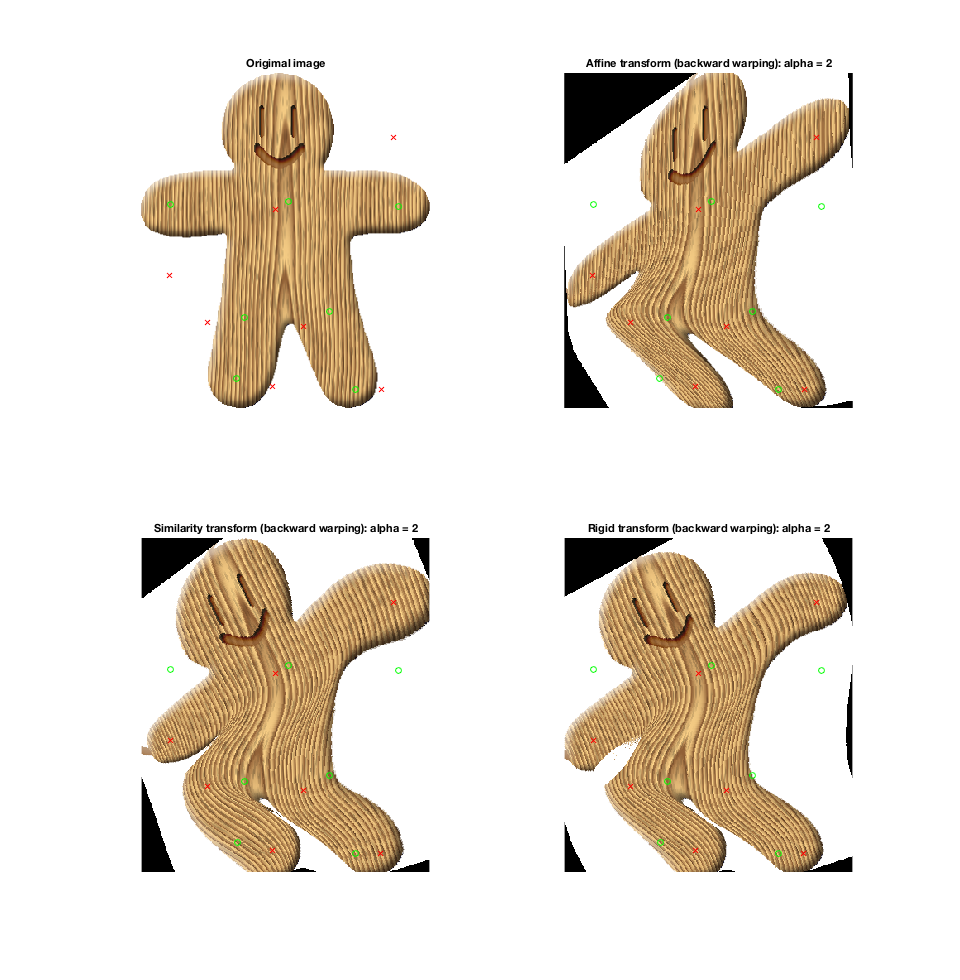
\includegraphics[width=0.7\textwidth]{deformation_backward_alpha2}}
\end{figure}

As the $\alpha$ increases, control points $\vec{p_i}$ tend to follow deformed points input $\vec{q_i}$ more. Finally, adapted the algorithm to another image which was carefully chosen :)

\begin{figure}[H]
\caption{kerr.jpg with $\alpha = 1.0$\label{fig:simple}}
\noindent\makebox[\textwidth]{
  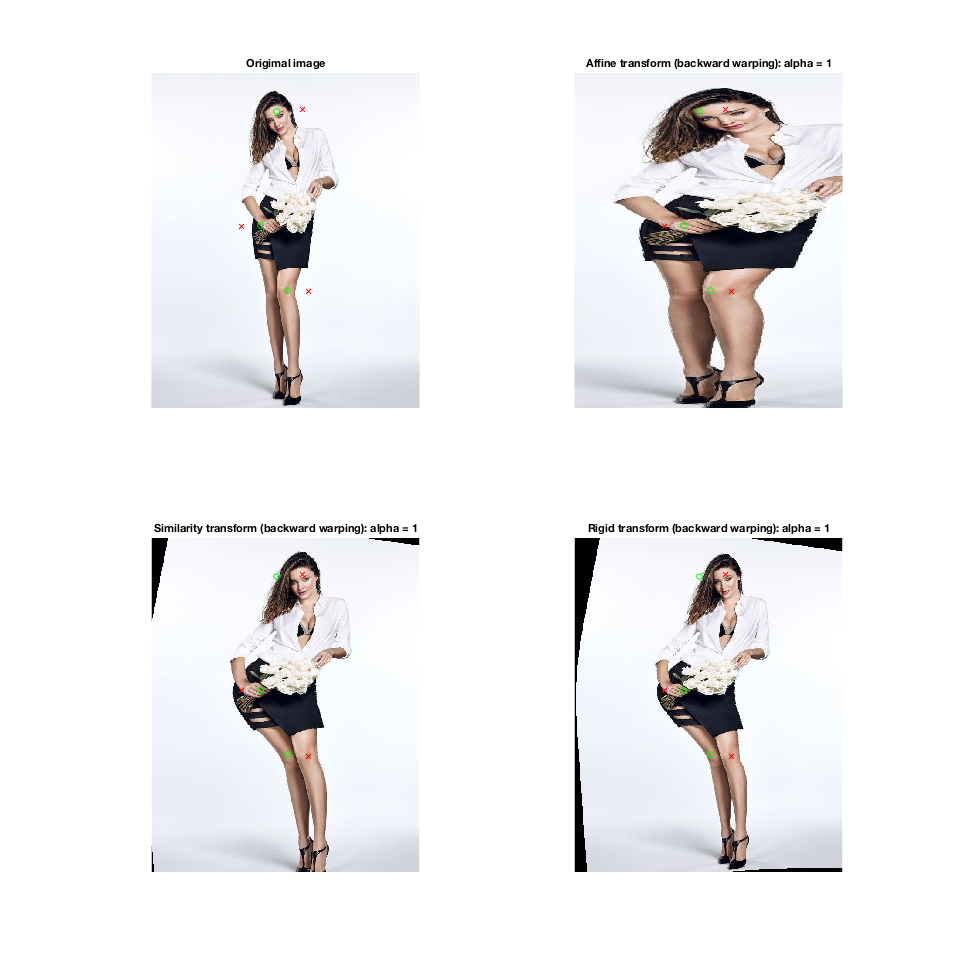
\includegraphics[width=\textwidth]{deformation_kerr}
}
\end{figure}

\vspace*{-0.5in}

%----------------------------------------------------------------------------------------
%	DISCUSSION
%----------------------------------------------------------------------------------------
\subsection{Discussion}

\begin{itemize}
	\item adapting backward warping, the artifacts (black dots) were disappeared. 
	\item as the $\alpha$ increases, control points $\vec{p_i}$ tend to follow deformed points input $\vec{q_i}$ more. $\alpha$ determines weight $w_i$ for each control point.
	\item rigid transformation is the most natural.  
\end{itemize}

\end{document}